\section{Experimental Results}

Our primary experimental results are a set of comparisons of tools using our method, for three languages: Solidity (the most popular language for smart contracts), Java, and Python.  We used the Universal Mutator tool for all experiments; for Solidity and Python, we believe the Universal Mutator is simply the best available tool.  For Java, PIT \cite{pitmut} is more popular, but does not produce source-level mutants, needed for PMD and for manual inspection of results.   Universal Mutator includes a large set of mutation operators, some unconventional (e.g., swapping order of function arguments) but based on real-world bugs; the complete set is described by regular expressions at \url{https://github.com/agroce/universalmutator/tree/master/universalmutator/static}.  However, most mutants that were detected came from a small set of  commonly-used operators \cite{mutant}, particularly 1) code deletion and 2) operator, conditional, and constant replacements.

We used our results to answer a set of research questions:

\begin{itemize}[labelsep=3pt,leftmargin=12pt]
\item {\bf RQ1:}  Does mutation analysis of static analysis tools produce actionable results?  That is, do raw mutation kills serve to distinguish tools from each other, or are all tools similar?
\item {\bf RQ2:}  Does our approach provide additional information beyond simply counting findings for the original, un-mutated analyzed code?  Do \emph{ratios} differ between tools?
\item {\bf RQ3:}  Do the rankings that raw kills and ratios establish agree with other sources of information about the effectiveness of the evaluated tools? 
\item {\bf RQ4:}  Do tools detect more mutants in programs for which they produce no warnings, initially?
\item {\bf RQ5:}  Are mutants distinguishing tools usually flagged due to real faults, where the finding is related to the introduced fault; that is, are our results usually \emph{meaningful}?
\item {\bf RQ6:}  Do individual mutants, prioritized for ease of examination, allow us to identify classes of faults that
  different tools are good at/bad at, and use this information to improve tools?  How does this compare to using mutants that have \emph{not} been prioritized?
  \end{itemize}

In particular, we consider {\bf RQ2} to be of critical importance; if the mutant ratios for tools differ, then this is clear evidence that our hypothesis that the tendency of mutants to be faults, and to expect that mutated code will, by a more precise and accurate tool, be flagged as problematic more often than non-mutated code, holds.  This expectation that (some subset of the) mutants can serve as proxies for real, detectable faults is the core concept of our approach.
{\bf RQ4} addresses a concern briefly mentioned in the introduction:  it is possible that warnings for the original code interfere with our definition of detection.  The ideal case for our approach is when a tool reports no findings for un-mutated code, and reports a finding when the mutant is introduced.  Chekam et al. showed that the ``clean program assumption'' for testing is a threat to the validity of investigations of the relationship between coverage and fault detection \cite{CleanProgram}, but we show that this is unlikely to be the case for our approach.  Our answer to {\bf RQ5} is somewhat inherently qualitative and incomplete; we cannot analyze all mutants on which results are based manually, and understanding the mutants and tool warnings completely would require deep understanding of all the subject programs.  However, in many cases, the impact of a mutant is clear, and the reason for warnings is obvious.  This was often enough the case that, as we discuss below, we are confident mutants that distinguish tools are meaningful (missed) opportunities for static analysis tools.
For {\bf RQ6}  we have only a preliminary answer.

\subsection{Solidity Smart Contract Tools}

\subsubsection{Smart Contracts and Smart Contract Static Analysis}

Smart contracts are autonomous code instruments, usually operating on a blockchain, that often have critical responsibilities such as facilitating and verifying (large) financial services transactions, tracking high-value physical goods or intellectual property, or even controlling ``decentralized organizations'' with multifarious aspects.  Security and correctness are thus critical in the smart contract domain, and static analysis is a key way to ensure allocation of high-value resources is not compromised.  The most popular smart contract platform, by far, is the Ethereum blockchain, and the Solidity smart contract language \cite{buterin2013whitepaper,wood2014yellow}; the Ethereum cryptocurrency has a market capitalization as we write of over \$100 billion dollars, largely fueled by interest in the smart contract functionality.  Ethereum contracts have been the targets of widely publicized attacks, with large financial consequences  \cite{spank,DAO}.   A recent paper examining results from 23 professional security audits of Solidity contracts argues that effective static analysis is a major key to avoiding such disasters in the future \cite{FC20}.

\subsubsection{Static Analysis Tools Compared}

%We analyzed three well-known tools for static analysis of Solidity smart contracts: Slither \cite{slither}\footnote{pip version 0.6.1}), SmartCheck \cite{smartcheck}\footnote{github commit 17fb98d9759eebeca1f92d48be52b85a1f5d8b89}, and Securify \cite{Securify}\footnote{github commit 0ffde61b9527be70b147d3ab687f11993d99212b}.

We analyzed three well-known tools for static analysis of Solidity smart contracts: Slither \cite{slither}, SmartCheck \cite{smartcheck}, and Securify \cite{Securify}.  Slither, based on an SSA-based intermediate language (SlithIR \cite{slither}) is an open-source tool from Trail of Bits.  SmartCheck, developed by SmartDec, translates Solidity source directly to an XML-based representation, then uses \emph{XPath} patterns to define problems.  Securify, from SRI Systems Lab at ETH Zurich, works at the bytecode level, first parsing and decompiling contracts, then translating to \emph{semantic facts} in order to look for problems.

\subsubsection{Smart Contract Selection}

We could have used a set of high-transaction contracts, or known-important contracts to validate our approach.  However, we knew that one of our goals in the Solidity experiments was to actually improve a mutation analysis tool, and the developers of the static analysis tools use exactly such benchmarks to validate their tools.  Basing our improvements on mutants of the contracts used for evaluation of proposed detectors would introduce a serious bias in our favor: we would be more likely to produce detectors that would have true positives and few false positives on the benchmark contracts.  We therefore instead selected 100 random contracts for which EtherScan (\url{https://etherscan.io/}) has source code, and used this (quite arbitrary) set of contracts from the actual blockchain to compare tools and identify opportunities for improvement.  The collected contracts had a total of 15,980 non-comment source lines, as measured by {\tt cloc}, with a mean size of 159.8 LOC and a median size of 108 LOC.  The largest single contract had 1,127 lines of code.  The Universal Mutator generated 46,769 valid mutants for these 100 contracts.

\subsubsection{Analysis Results}

\begin{figure}
  \centering
  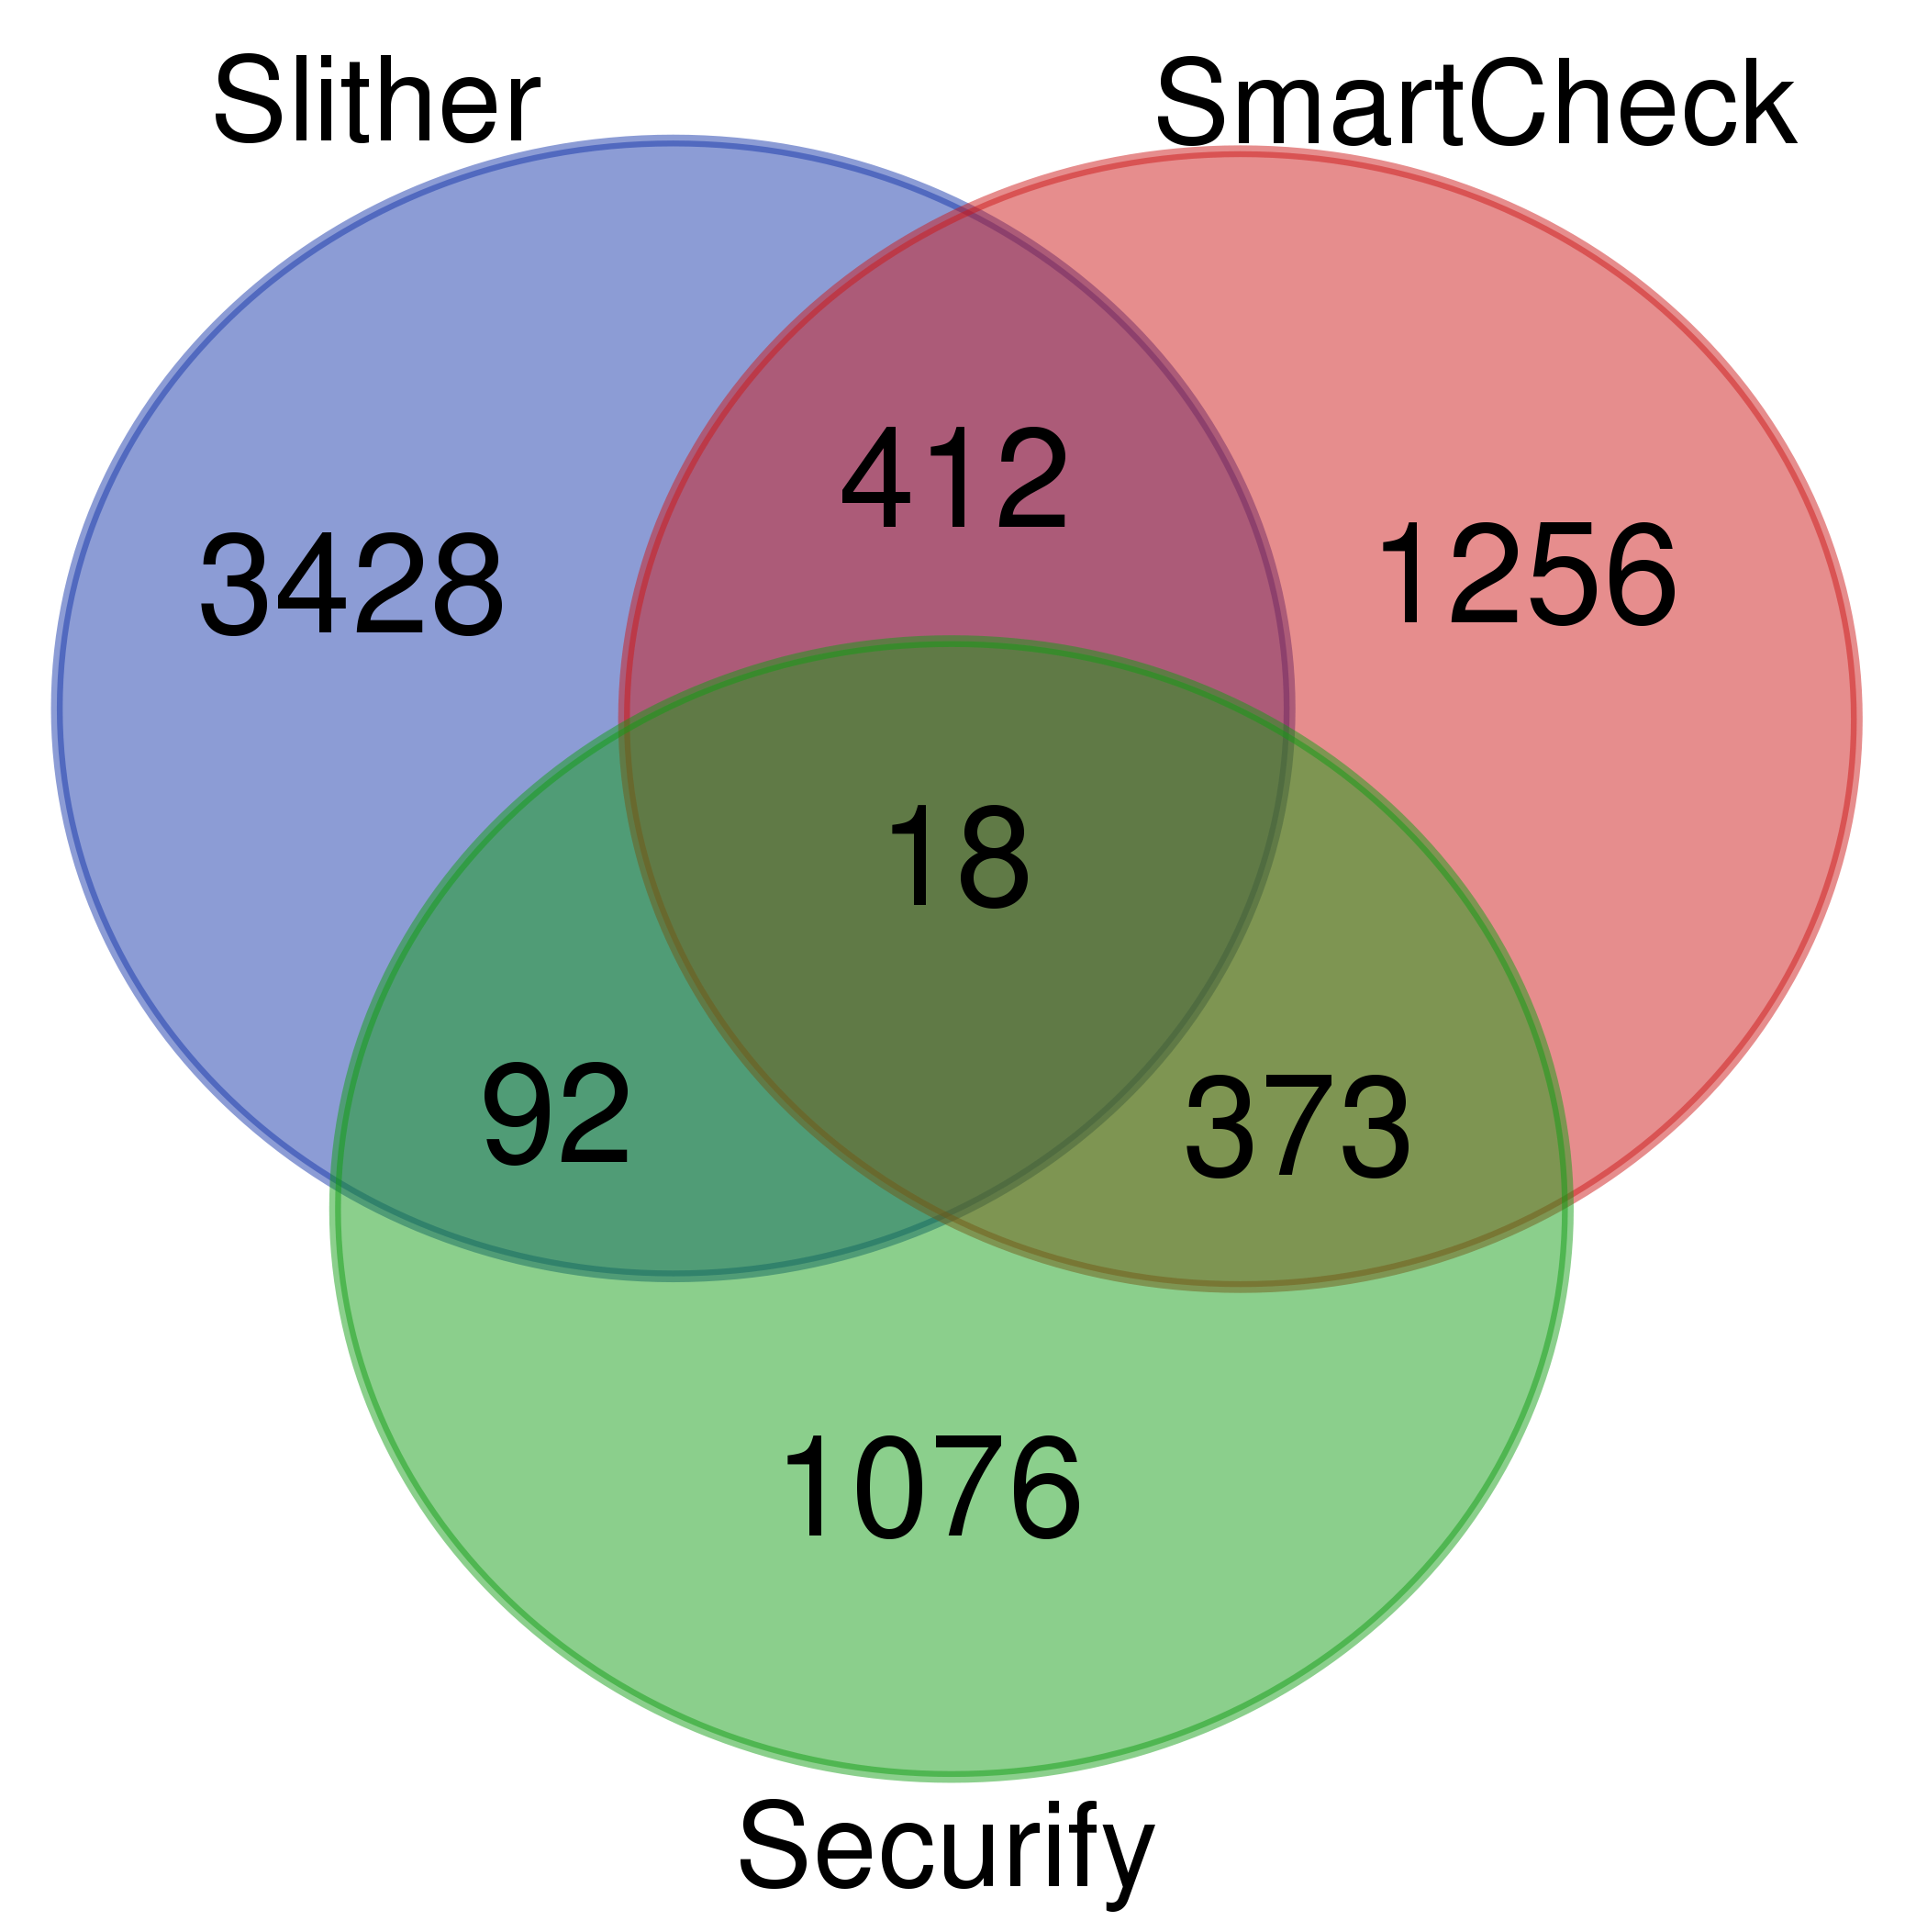
\includegraphics[width=0.35\columnwidth]{solidity.png}
  \caption{Mutants killed by Solidity static analysis tools.}
  \label{fig:solidityvenn}
\end{figure}

\begin{table}
  \begin{tabular}{l|r|r|r|r|r}
    & \multicolumn{2}{|c|}{Findings} & \multicolumn{2}{|c|}{Mutation Score}  & Mutant \\
    Tool & Mean & Median & Mean & Median & Ratio\\
    \hline
    \hline
    Slither & 2.37 & 1.0 & 0.09 & 0.09 & 0.038 \\
    Clean (39) & - & - & 0.11 & 0.11 & -\\
    \hline
    SmartCheck & 1.89 & 1.0 & 0.05 & 0.05 & 0.026 \\
    Clean (27) & - & - & 0.03 & 0.01 & - \\
    \hline
    Securify & 24.65 & 17.0 & 0.03 & 0.02 &  0.001 \\
    Clean (5) & - & - & 0.00 & 0.00 & - \\
    \hline
    
  \end{tabular}
  \caption{Solidity tool results over all contracts.}
  \label{tab:scoresolidity}
\end{table}


Figure \ref{fig:solidityvenn} shows the mutants killed by the Solidity analysis tools.  Table \ref{tab:scoresolidity} provides numeric details of the results, including the \emph{ratio} for each tool, adjusting its mutation scores by its' general tendency to produce findings.  The second row for each tool shows the number of contracts for which it reported no findings, and the mutation scores over those contracts, only. A user examining these results would suspect that Slither and SmartCheck are both useful tools, and should likely both be applied in a high-risk security-sensitive context like smart contract development.  A user might also suspect that the large number of findings produced, and smaller number of mutants killed, for Securify, means that whether to apply Securify is a more difficult decision.  On the one hand, Securify does detect nearly as many mutants it alone can identify as SmartCheck.  The large number of findings, and very bad mutant ratio, however, lead us to suspect that many of these ``detected'' mutants are false positives (or, at least, that the problem is not the one Securify identifies).  Extracting the signal from Securify's noise will be difficult.  We also note that while running Slither and SmartCheck on all 46,769 valid mutants was relatively quick (it took about 6 days sequential compute time for Slither and 3 days for SmartCheck, i.e., about 5-15 seconds per mutant for both tools), Securify often required many hours to analyze a mutant, and frequently required a few days to analyze a mutant; the full analysis required over three months of compute time.  However, similar statistical results would almost certainly be produced by running as few as 1,000 mutants, randomly selected, due to the implications of Tchebysheff’s inequality \cite{gopinath2015hard}, a technique that should improve scalability for all such analyses.

If we consider results at the individual contract level, the overall picture is in some ways even clearer.  Slither detected more mutants than Securify for 84 of the contracts, and more than SmartCheck for 85 of the contracts.  SmartCheck detected more mutants than Securify for 83 of the contracts.  Comparing ratios instead, Slither was better than Security for 97 contracts, but better than SmartCheck for only 75 of the contracts.  SmartCheck's ratio was better than Securify's for 95 contracts.  The standard deviation of contract raw scores was 0.05 for Slither, 0.03 for SmartCheck, and 0.04 for Securify.

For our research questions, {\bf RQ1} is clearly answered in the affirmative.  Figure \ref{fig:solidityvenn} shows that the tools address quite different problems, with all tools reporting far more uniquely detected mutants than mutants in common with other tools.  There are only 18 mutants detected by all tools, all of them involving replacement of {\tt msg.sender} (the caller of a smart contract, which may be another smart contract) with {\tt tx.origin} (the original initiator of a sequence of blockchain calls, a ``human'' account).  Use of {\tt tx.origin} is often (though not always) a bad idea, and can lead to incorrect behavior, so it is not surprising tools all recognize some misuses of it.

{\bf RQ2} is also answered in the affirmative.  Counting findings for un-mutated code might suggest that Securify is the best tool, by a wide margin, but in the context of its near-zero mutant ratio, we must suspect (and we partially manually confirmed) that many of the warnings are false positives.  Slither has the best mutant ratio, but the margin between it and SmartCheck confirms that both tools likely provide value; we note there is a 25\% chance that SmartCheck has a better ratio than Slither for an individual contract.

For {\bf RQ3}, there are only a few tool comparisons in the literature; this is probably due to the fast-moving nature of the blockchain analysis world; the oldest of these tools' publication dates is 2018.  The most extensive is that of Durieux et al. \cite{durieux2019empirical}, though it unfortunately was unable to provide anything other than an implicit look at false positives, somewhat limiting its practicality.  Slither detected 17\% of known vulnerabilities in their analysis, vs. 11\% for SmartCheck and 9\% for Securify. Slither and SmartCheck were also among the four (out of 9) tools that detected vulnerabilities in the most categories; Securify was not.  The overall recommendation of Durieux et al. was to use a combination of Slither and Mythril \cite{mythril-code} for contract analysis.  Parizi et al. \cite{Parizi} also offer a ranking of tools, and determined that SmartCheck was the most effective, and far more so than Securify; unfortunately, they did not include Slither in their set of evaluated tools.

The Slither paper \cite{slither} also provides an evaluation of all three tools.  Their findings counts differ from ours because of different choices (we threw out merely informational results), but these are unrelated to mutation analysis, in any case.  The evaluation only considered reentrancy faults \cite{SurveyAttacks,FC20} (which are sometimes, but only rarely, introduced by mutants).  For reentrancy, Slither performed best on two real-world large contracts, finding subtle bugs in both, SmartCheck detected the problem in one of the two, and Securify detected neither.  For a set of 1,000 contracts, SmartCheck had a high false positive rate (over 70\%) but detected more actual reentrancies (209) than Slither (99) or Securify (6).  On the other hand, Slither's low false positive rate of 11\%  makes its results possibly more useful in practice.

For {\bf RQ4}, on the changes seen when restricting analysis to clean contracts, Slither did slightly better at detecting mutants when the original contract was clean for Slither, and the other two tools did somewhat worse on contracts for which they reported no findings.  For the three contracts clean for all tools, Slither performed almost exactly as it did over contracts in general, and the other tools performed worse, by about the same margin as they did for their own clean contracts.  For our approach, we only need a weak version of the ``clean program assumption'':  the threat is that kills may be under-reported for non-clean programs, due to interference with findings for the original code.  It is not a problem if mutation scores are \emph{worse} for programs where a tool reports no findings for the un-mutated code.  We therefore, for smart contracts, find no threat to our approach arising from the presence of findings on un-mutated code.  We speculate that ``clean'' results for some tools result from contracts where the tool has trouble with the contract code, but does not actually crash; Slither may do better on clean code because it has fewer such failures, and clean contracts are probably somewhat easier to analyze.

Following the method proposed in Section \ref{sec:method},  for {\bf RQ5} we focused on examining mutants detected by at least one tool, but not detected by all tools, the only ones that actually influence the comparison of tools.  The vast majority of the mutants in this set were meaningful semantic changes a static analysis tool could be expected to detect, and the findings produced by tools were relevant to the nature of the fault.  We do not believe that \emph{all} mutants represent definite faults; some are harmless but unusual code changes.  Many cases where use of {\tt tx.origin} in place of {\tt msg.sender} was flagged seem to us to be strange, but not necessarily incorrect, code.  On the other hand, it is not at all unreasonable for tools to report such notably strange code.   Our estimate is that, ignoring {\tt tx.origin} cases, \emph{at least 70\% of the mutants detected by one, but not all, tools, represent realistic bugs}, and failure to detect is roughly equally due to missing detectors and imprecise analysis.

Because our random contracts' quality might be low, we also checked our results on 30 contracts from the Solidity documentation, the \emph{Mastering Ethereum} book \cite{masteringEth}, and a handful of selected, recent, higher quality blockchain contracts.  Slither had a mean mutation score of 0.11, vs. 0.04 for SmartCheck and 0.01 for Securify.  Associated mutant ratios were 0.38, 0.08, and 0.007.  Mutant kill overlap was also similar; in fact, Figure \ref{fig:examplevenn} shows the results: Slither is A, SmartCheck is B, and Securify is C.

\subsubsection{Improving Slither {\bf (RQ6)}}

Based on the differential mutation analysis, we identified three low-hanging fruit to improve the performance of Slither.  We chose Slither in part because it seems to have a better underlying intermediate language and analysis engine, and thus is likely to produce better results for the same rule than the other tools.  The process was simple.  First, we produced a list of all mutants killed by either SmartCheck or Securify, but not killed by Slither.  We then applied the prioritization method based on the FPF algorithm and the distance metric described in Section \ref{sec:prioritizing}, and examined the mutants in rank order.  Many of the mutants were difficult to identify as true or false positives, absent context.  Some opportunities for enhancement were clear, but seemed likely to require considerable effort to implement without producing a large number of false positives.  For example, Securify often detected when an ERC20 token contract's guard preventing making the special 0x0 address the owner of a contract was removed, and issued the error {\tt Violation for MissingInputValidation}. Detecting such missing guards is probably useful, but doing so without producing false positives is non-trivial.  We wanted to show that mutants could identify \emph{useful} but \emph{easy to implement} missing detectors.  Examining only a few mutants, we identified three:

\begin{figure}
  {\scriptsize
      {\bf Mutant showing Boolean constant misuse.}

    
\noindent
\begin{verbatim}
  if (!p.recipient.send(p.amount)) \{  // Make the payment
  ==>          if (true) \{  // Make the payment
  if (true) \{  // Make the payment
\end{verbatim}
}

 {\scriptsize
 {\bf Mutant showing Type-based tautologies.}
\begin{verbatim}
  require(nextDiscountTTMTokenId6 >= 361 \&\& ...);
  ==>  ...361...==>...0...
  require(nextDiscountTTMTokenId6 >= 0 \&\& ...);
\end{verbatim}
}


      {\scriptsize
      {\bf Mutant showing Loss of precision.}        
\begin{verbatim}
  byte char = byte(bytes32(uint(x) * 2 ** (8 * j)));
  ==>  ...*...==>.../...
  byte char = byte(bytes32(uint(x) * 2 ** (8 / j)));
\end{verbatim}
}
        \caption{Examples of mutants leading to new detectors.}
       \label{fig:newdetect}
    \end{figure}

\begin{enumerate}
\item {\bf Boolean constant misuse:}  This detector flags code like {\tt if (true)} or {\tt g(b || true)} (where {\tt g} is a function that takes a Boolean input).  Constant-valued conditionals tend to indicate debugging efforts that have persisted into production code, or other faults; there are almost no circumstances where a conditional should not vary with state or input.  This detector is actually split into two detectors, one for this serious issue, and an informational/stylistic detector that flags code such as {\tt if (x == true)}, which is merely difficult to read.

\item {\bf Type-based tautologies:}  A type-based tautology is again a case where a Boolean expression has a constant value, but this is not due to misuse of a Boolean constant, but is instead due to the \emph{types} in a comparison.  For example, if {\tt x} is an unsigned integer type, the comparison {\tt x >= 0} is always true and {\tt x < 0} is always false.  This detector is a generalization of the SmartCheck detector \url{https://github.com/smartdec/smartcheck/blob/master/rule\_descriptions/SOLIDITY\_UINT\_CANT\_BE\_NEGATIVE/}, modified to actually compute the ranges of types and identify other cases such as {\tt y < 512} where {\tt y}'s type is {\tt int8}.

\item {\bf Loss of precision:}  Solidity only supports integer types, so performing division before multiplication can introduce avoidable rounding.  This is a fairly important problem, given Solidity code often performs critical financial calculations.  SmartCheck provides a detector for such precision losses \url{https://github.com/smartdec/smartcheck/blob/master/rule\_descriptions/SOLIDITY\_DIV\_MUL/}.
\end{enumerate}      

All three of these detectors were submitted as PRs, vetted over an internal benchmark set of contracts used by the Slither developers to evaluate new detectors, and accepted for release in the public version of Slither.  All three detectors produce some true positives (actual problems, though not always exploitable) in benchmark contracts, have acceptably low false positive rates, and were deemed valuable enough to include as non-informational (medium severity) detectors.  The first mutants in prioritized rank exhibiting the issues, shown above, were the 2nd, 9th, and 12th non-statement-deletion mutants ranked for SmartCheck, out of over 800 such mutants.  Using our prioritization, it was possible to identify these issues by examining fewer than 20 unkilled mutants.  Without prioritization, on average a developer would have to look at more than 200, 80, and 400 mutants, respectively, to find instances of these problems.  Interestingly, the very fact that these instances are ``needles in a haystack'' among the mutants not killed by Slither means that the results in Figure \ref{fig:solidityvenn} and Table \ref{tab:scoresolidity} are almost unaltered by our improvements to Slither: our analysis is fairly robust to modest tool improvements, unless added detectors account for a large number of mutants not detected by the tool.  Adding such detectors will also only improve mutation ratio if they do not add many false positives.  Substantial changes in results therefore require adding very effective (for mutants) detectors that seldom trigger for correct code (or at least trigger much less than for mutants).  ``Cheating'' with respect to a mutation benchmark is thus, we hope, very difficult.

There were 92 separately ranked statement deletion mutants also.  These, however, could all be ignored, as they were almost entirely duplicates related to the missing-return statement detector.  If this detector were not already present as a private Slither detector, it would also be a good candidate for addition to the tool.  Our three submitted detectors were not present as private detectors, and only one (the type-based tautology detector) had even been identified, via a GitHub issue, as a potential improvement (and only in the private version of Slither).  Combining statement deletion mutants with other mutants only moved the mutants we used down to 3rd, 11th, and 14th positions.  By default we rank statement deletions separately, since such mutants are usually easier to understand and evaluate, and in testing (but not static analysis) they are likely to be the most critical faults not detected.

Examining the first 100 mutants in the unprioritized lists for SmartCheck and Securify, ordered by contract ID and mutant number (roughly source line mutated) we were unable to identify \emph{any} obviously interesting mutants, suggesting that it is indeed hard to use mutation analysis results without prioritization. A large majority of the mutants we inspected involved either the missing
{\tt return} problem noted in the introduction, or replacing {\tt msg.sender} with {\tt tx.origin}; Slither has a detector for misuses of {\tt tx.origin}.  SmartCheck and Securify tend to identify most (though not all) uses of {\tt tx.origin} as incorrect, while Slither has a more selective rule, intended to reduce false positives.
It is hard to scale our efforts here to a larger experiment, since writing and submitting changes to static analysis tools is always going to be a fairly onerous task, but we believe that our successful addition of new detectors, and the ease of identifying candidate detectors using mutant prioritization supports a limited affirmative answer to {\bf RQ6}.

\subsection{Java Tools}

\subsubsection{Static Analysis Tools Compared}

For Java, we again compared three tools.  SpotBugs (\url{https://spotbugs.github.io/}) is the ``spiritual successor'' of FindBugs \cite{FindBugs,CompareJavaTools}.  PMD (\url{https://pmd.github.io/}) \cite{CompareJavaTools} is an extensible cross-language static code analyzer.  FaceBook's Infer (\url{https://fbinfer.com/}) \cite{Infer} focuses on diff-related detection of serious errors (concurrency, memory safety, and information flow).

\subsubsection{Project Selection}

For Java and Python, we did not have to worry about invalidating tool improvements by basing our results on benchmark code.  We therefore aimed to use realistic, important source code.  We selected top GitHub projects (defined by number of stars) for each language, and removed projects with fewer than 5 developers or less than six months of commit history (as well as projects that did not build).  For Java, we analyzed the top 15 projects satisfying our criteria, with a maximum of 623,355 LOC and a minimum of 3,957 LOC, and a total size of 1.8 million LOC.  Because the Universal Mutator does not ``know'' Java syntax, and Java is very verbose, the Java compiler rejected a large number of the generated mutants (e.g., deleting declarations).  We still, due to the huge size of the source files and thus number of mutants (and time to compile full projects), restricted our analysis to files where Universal Mutator's implementation of TCE \cite{TCE} for Java was useful, i.e. individual files that could be compiled and the bytecode compared, leaving us with just over 70,000 mutants, ranging from 136 to 10,016 per project.

\subsubsection{Analysis Results}


\begin{figure}
  \centering
  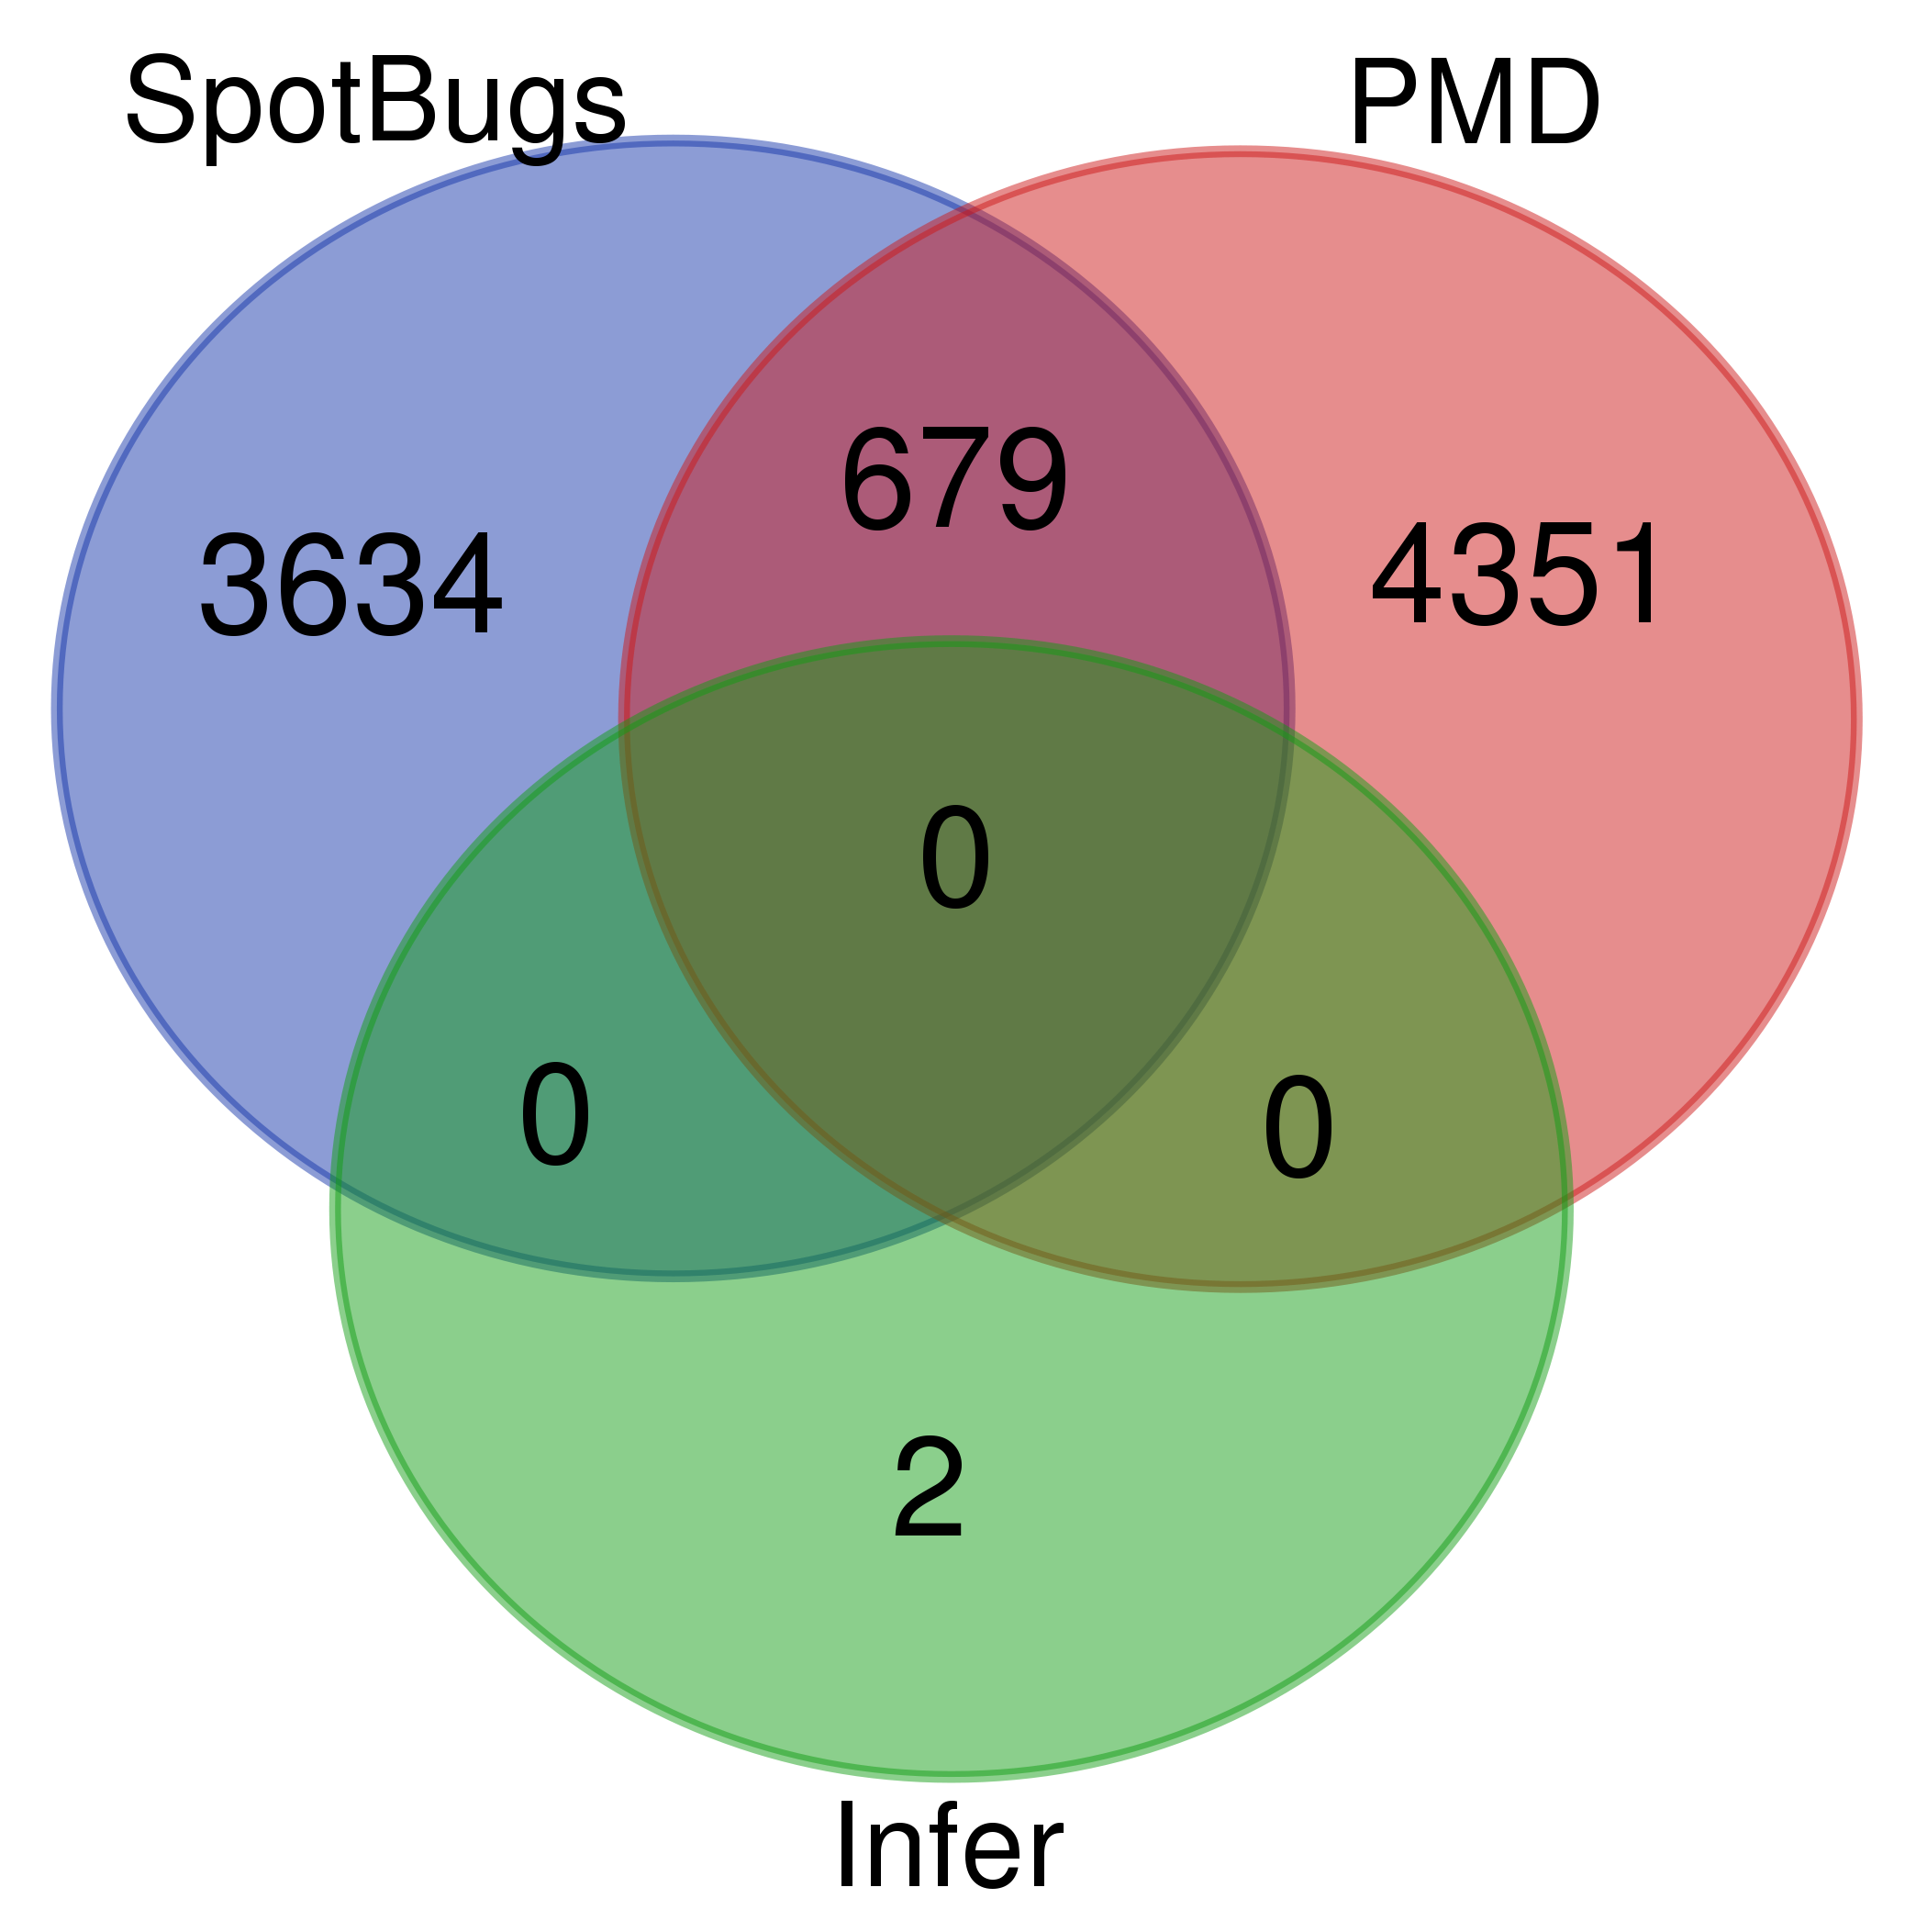
\includegraphics[width=0.30\columnwidth]{java.png}
  \caption{Mutants killed by Java static analysis tools.}
  \label{fig:javavenn}
\end{figure}

\begin{table}
  \begin{tabular}{l|r|r|r|r|r}
    & \multicolumn{2}{|c|}{Findings} & \multicolumn{2}{|c|}{Mutation Score}  & Mutant \\
    Tool & Mean & Median & Mean & Median & Ratio\\
    \hline
    \hline
    SpotBugs & 28.93 & 14.00 & 0.07 & 0.07 & 0.002 \\
    Clean (3) & - & - & 0.05 & 0.06 - \\
    \hline
    PMD & 53.73 & 32.00 & 0.07 & 0.07 & 0.001 \\
    Clean (0) & - & - & - & - & - \\
    \hline
    Infer & 11.60 & 3.00 & 0.00 & 0.00 &  0.000 \\
    Clean (6) & - & - & 0.00 & 0.00 \\
    \hline
  \end{tabular}
  \caption{Java tool results over all projects.}
  \label{tab:scorejava}
\end{table}



Figure \ref{fig:javavenn} shows the mutants killed by the Java analysis tools, and Table \ref{tab:scorejava} provides numeric results for projects and clean projects, respectively.  At the individual project level, Infer was never best; PMD had a better raw score than SpotBugs for 10/15 projects, but SpotBug had a better \emph{ratio} for 11.  There is likely a tradeoff between verbosity and precision.  Standard deviation in project scores was 0.05 for SpotBugs, 0.04 for PMD, and 0 for Infer.

In terms of {\bf RQ1}, the raw kills results suggest there is considereable value in running both SpotBugs and PMD.  Both produce a large number of unique detections, though PMD produces about 20\% more than SpotBugs.
Infer on the other hand, is only able to detect two mutants, but these are unique; both were, however, spurious concurrency warnings.  It may be that the diff sizes in our code were simply too small for Infer's approach.
{\bf RQ2} is also answered in the affirmative.  While the raw kills for SpotBugs are not as good as for PMD, it had fewer findings, giving it a mutant ratio approximately twice that of PMD.

We note that SpotBugs crashed for many more Java programs than PMD and Infer (neither crashed for any original file in our experiments).  SpotBugs ``failed to detect'' 23,000 of the mutants because it did not process the un-mutated file for 383 files, over 12 of the 15 projects---just over 23\% of the 1,664 total files.  Removing files for which SpotBugs failed, however, did not dramatically change results; SpotBugs' mean mutation score rose to 0.09, and mutant ratio rose to 0.003, but PMD's mean score rose to 0.10, and mutant ratio to 0.002.

\begin{figure}
  {\scriptsize
    % \begin{itemize}
    \raggedright    
  \url{https://stackoverflow.com/questions/4297014/what-are-the-differences-between-pmd-and-findbugs} \\
  \url{https://www.sw-engineering-candies.com/blog-1/comparison-of-findbugs-pmd-and-checkstyle} \\
  \url{https://www.reddit.com/r/java/comments/3i7w6n/checkstyle_vs_pmd_vs_findbugs_for_dummies_why/} \\
  %\end{itemize}
  }
\caption{Discussions of Java static analysis tools.}
\label{fig:blog}
\end{figure}

For {\bf RQ3}, to our knowledge there is no academic comparison of all three tools; one study dates from 2004 \cite{CompareJavaTools}, used FindBugs, not SpotBugs, and reached no strong conclusions with respect to FindBugs vs. PMD; a more recent study found that SpotBugs outperformed Infer for Defects4J \cite{just2014defects4j} bugs \cite{AllBugs}, but did not compare to PMD.  However, the user postings listed in Figure \ref{fig:blog}, plus personal communications with security analysts who use these tools \cite{personalJava} supported some basic conclusions.  SpotBugs is perhaps the best tool for finding bugs; PMD focuses more on stylistic issues and has a weaker semantic model.  Running both is definitely recommended, as neither is extremely effective.  Infer is closer to a model checker focusing on resource leaks than a truly general-purpose tool, arguably.  In fact, we suspect Infer would perform much better if we used mutation operators targeting some important subtle Java bugs; Infer is probably not a good \emph{general-purpose} static analysis tool for Java.  Note that we did not use Infer's experimental detectors.
For {\bf RQ4} there were very few clean projects, but we see no evidence that non-clean code is a source of degradation in mutation detection.

For Java, again, the large majority ($>$ 75\%) of randomly chosen mutants in the tool difference set we inspected for {\bf RQ5} were definitely meaningful, essentially ``real faults.''  In particular, for Java, the large majority of mutants involved either deleted method calls or changes to conditionals (e.g., {\tt == null} to {\tt != null}) that would clearly introduce potential null pointer exceptions (NPEs), and such a possible NPE was the produced finding.  While the differences between Solidity tools were often due to different detectors, the Java differences seemed mostly rooted in analysis engine methods; all tools aim to warn about potential NPEs.  Because the number of mutants we could examine and understand was smaller, we are less confident in making a probabilistic estimate than with Solidity, but it was clear the basis of the comparison was primarily realistic faults, which some tools detected and others did not.

\subsection{Python Tools}

\subsubsection{Static Analysis Tools Compared}

We compared three widely used and well-known Python tools:  Pylint \url{https://www.pylint.org/} (probably the most widely used of Python bug finding tools), pyflakes \url{https://pypi.org/project/pyflakes/}, designed to be faster, lighter-weight, and more focused on bugs (without configuration) than Pylint, and PyChecker \url{http://pychecker.sourceforge.net/}, an older, but still used tool.

\subsubsection{Project Selection}

For Python, we analyzed the top 25 GitHub projects by our criteria (see above), due to the smaller size of Python projects.  These ranged in size from 137 LOC to 29,339 LOC, with a total size of about 75 KLOC, and a mean size of 3,185 LOC.  We analyzed 158,418 valid, non-TCE redundant, mutants taken from these programs.

\subsubsection{Analysis Results}


\begin{figure}
  \centering
  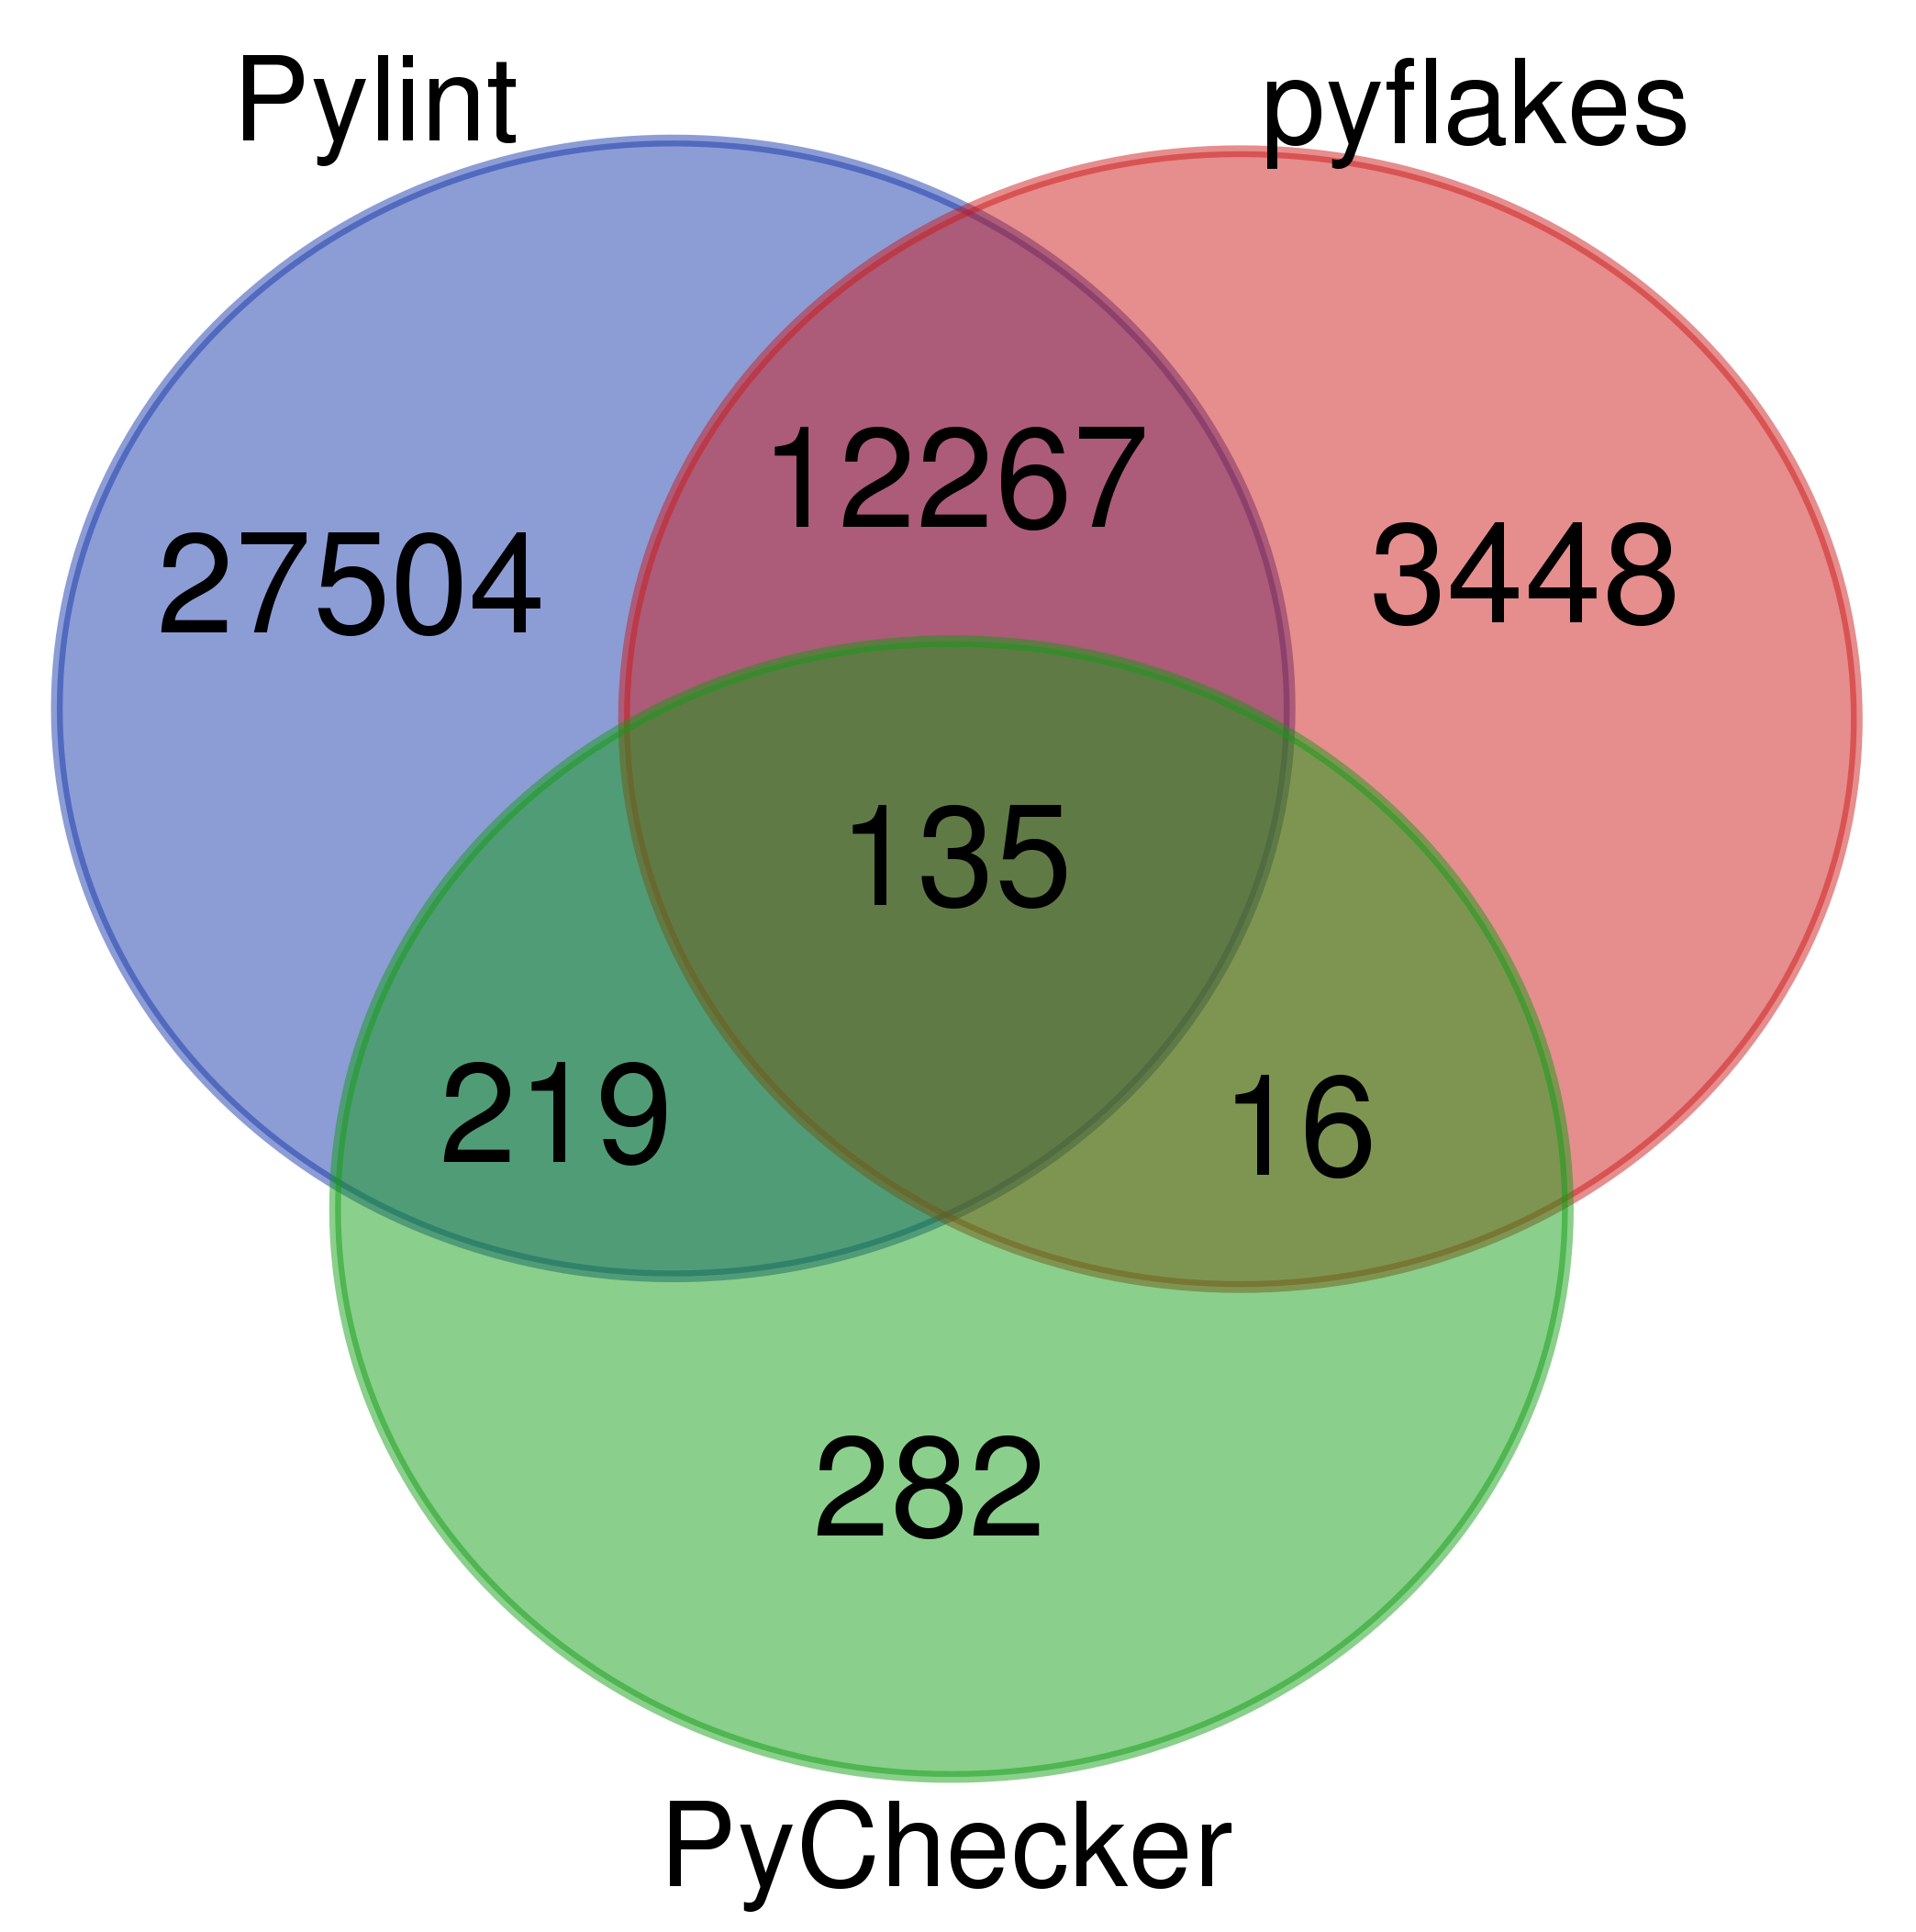
\includegraphics[width=0.30\columnwidth]{python_new.png}
  \caption{Mutants killed by Python static analysis tools.}
  \label{fig:pythonvenn}
\end{figure}

\begin{table}
\begin{tabular}{l|r|r|r|r|r}
& \multicolumn{2}{|c|}{Findings} & \multicolumn{2}{|c|}{Mutation Score} & Mutant \\
Tool & Mean & Median & Mean & Median & Ratio\\
\hline
\hline
Pylint & 10.63 & 5.50 & 0.31 & 0.34 & 0.03 \\
Clean (4) & - & - & 0.49 & 0.47 & - \\
\hline
pyflakes & 1.46 & 0.00 & 0.14 & 0.12 & 0.09 \\
Clean (14) & - & - & 0.14 & 0.12 & - \\
\hline
PyChecker & 11.6 & 0.00 & 0.01 & 0.00 & 0.00 \\
Clean (4) & - & - & 0.00 & 0.00 & - \\
\hline
\end{tabular}
\caption{Python tool results over all projects.}
\label{tab:scorepython}
\end{table}

Figure \ref{fig:pythonvenn} shows the mutants killed by the Python analysis tools, and Table \ref{tab:scorepython} provides numeric results for projects and clean projects, respectively.  At the project level, Pylint was better than pyflakes and PyChecker for 21 and 24 projects, respectively, by raw score; pyflakes was better than Pylint and PyChecker for 3 and 24 projects, respectively; PyChecker was never better than another tool by raw score.  Switching to ratio measures, Pylint was better than pyflakes and PyChecker for 11 and 23 projects, respectively; pyflakes was better than Pylint and PyChecker for 13 and 24 projects, respectively.  PyChecker was better than Pylint for one project, by ratio.  
Standard deviations in mutation scores were sometimes high for Python:  0.17 for Pylint, 0.08 for pyflakes, and 0.01 for PyChecker.

For {\bf RQ1}, there is a clear difference between tools.  Pylint uniquely kills almost an order of magnitude more mutants than the next-best tool.  There is a large overlap between Pylint and pyflakes, while PyChecker is both much less effective and doing something fairly different than the other tools.  From the diagram, one might think that pyflakes acts, to some extent, as a less verbose ``subset'' of Pylint, in that most mutants detected by pyflakes are also detected by Pylint (however, the nearly 3,500 killed mutants unique to pyflakes suggest it is a useful tool, perhaps most useful after problems also reported by Pylint are fixed).  PyChecker performs poorly in part because it crashed (due to changes in Python since the last update to the tool) for 19 of the 25 projects; however, it also performed poorly on programs where it worked.

The mutant ratios {\bf RQ2} show that pyflakes is more competitive than is obvious from raw kill comparisons.  The mutant ratio is almost three times as good as for Pylint!  That is, some of Pylint's advantage may be due to general verbosity, even once stylistic warnings are turned off.   Combining the results from raw kills and ratios, a strategy of using pyflakes as a quick check for problems, then using both pyflakes and Pylint for more in-depth analysis makes sense.  Whether to use both pyflakes and Pylint in CI is a rquestion of tolerance for handling false positives, but it is clear that the ``price'' of additional warnings from Pylint is (1) high but (2) not without ereturn on investment (in terms of additional real finds).  PyChecker is probably too outdated, and sometimes too verbose when it works, to be useful.
 
\begin{figure}
  {\scriptsize
    % \begin{itemize}
    \raggedright
  \url{https://stackoverflow.com/questions/1428872/pylint-pychecker-or-pyflakes}\\
  \url{https://www.reddit.com/r/Python/comments/ii3gm/experience_with_pylint_pychecker_pyflakes/}\\
  \url{https://www.slant.co/versus/12630/12631/~pylint_vs_pyflakes}\\
  \url{https://news.ycombinator.com/item?id=12748885}\\
  \url{https://doughellmann.com/blog/2008/03/01/static-code-analizers-for-python/}\\
  %\end{itemize}
  }
\caption{Discussions of Python static analysis tools.}
\label{fig:blogpython}
\end{figure}

For {\bf RQ3}, there were again no academic comparisons we could find.  However, opinions on the web were quite common (see Figure \ref{fig:blogpython}, which lists ones we examined).  It is hard to summarize the overall opinion here, since it ranges considerably.  There is probably general agreement that PyChecker is old and maybe less useful, but also terse and sometimes helpful.  Pylint is the most recommended tool, and the general complaint that it is too picky was somewhat mitigated in our results by turning off warnings that are clearly purely stylistic.  Pyflakes is also well liked, and is considered much less verbose than Pylint; this was definitely reflected in our results, where Pyflakes underperformed in raw kills, but had a much better mutant ratio than Pylint.
For {\bf RQ4}, Pylint performed significantly better on clean projects.  Performance for the other two tools was essentially unchanged.

For Python, all but three of the mutants we examined for {\bf RQ 5} (a random sample of 100 mutants with a kill difference) involved code changes we agreed were definitely buggy, and would cause incorrect behavior if executed (the exceptions were deletions of code with no effect on state, e.g., strings as comments).  The large majority involved statement deletions, detected via 1) unused variables/arguments, 2) instances lacking a member field, or 3) undefined variables.  Interestingly, this seems to be an engine issue more than a detector issue, as pyflakes and Pylint both basically support all of these kinds of checks.  In some cases the two tools both detected a problem (but PyChecker did not) but differed as to \emph{which} variable was not used or defined, again suggesting an engine rather than detection rule difference.  Pylint's better performance was mostly, in the sample, due to detecting more of these issues, though it also was the only tool in the sample that detected arithmetic operation changes, due as far as we could determine to constant index changes.  Pylint also detected a few mutants no other tool did, due to the presence of unreachable code.  In one case, it also noticed a protected member access via a change in constant index, a surprisingly complex problem to find, in our opinion.  PyChecker was never the sole detecting tool for any mutants in our sample.

\subsection{Threats to Validity}

The primary threat to validity in terms of generalization is that we only examined nine static analysis tools, and our analyses were restricted to 100 smart contracts, 15 Java projects, and 25 Python projects.   Because it is hard to identify a ground truth to compare with (the motivation for our approach), we cannot be certain that our rankings of tools are correct even for these tools and this code.  However, where there are existing discussions of the tools, our results seem to agree with these, but add substantial detail.

We used the Universal Mutator \cite{universalmutator,regexpMut}, which aggressively produces large numbers of mutants, but does not target any particular software defect patterns, to generate all mutants.
There is no room in the paper to present the exact set of projects analyzed, but we have provided an (anonymized) github repository containing raw results for inspection by reviewers, or further analysis by other researchers (\url{https://github.com/mutantsforstaticanalysis/rawdata}).
